\section{Neural network based caching policy}

\subsection{Architecture}

\begin{figure}[b!]
	\centering
	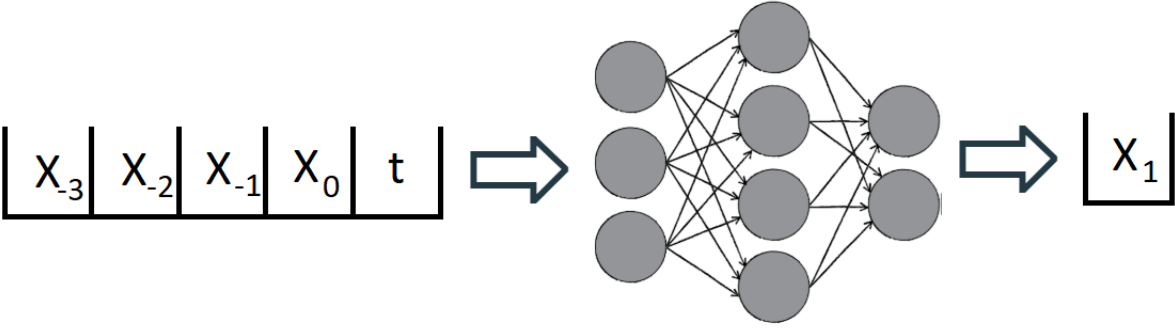
\includegraphics[width=\linewidth]{pics/cache1.png}
	\caption{Neural network architecture for caching policy.}
	\label{fig:cache1}
\end{figure}

Following the success in the application of a neural network for object popularity predictions, we are proposing a neural network based caching policy. On the Figure \ref{fig:cache1} you can see the proposed usage of the neural network by the policy.

\begin{itemize}
	\item $X_{-3}$ through $X_{-1}$ are popularities of the object in the previous 3 time frames;
	\item $X_0$ is the popularity of the object in the current time frame;
	\item $t$ is the fraction of the current time window that has already passed;
	\item $X_1$ is the popularity of the object in the future;
\end{itemize}

As you can see, the architecture of the neural network is slightly different from the one described in the previous section.  The difference is caused by the nature of the application of caching policies. The policy is working in the real-time thus we cannot operate in the framework of only previous and next time frames. $X_0$ represents the popularity in the current time frame. But at the beginning of the time frame, the quality of the value $X_0$ may be low since there will not be enough requests in the time window to estimate the popularity with reasonable accuracy. To help with this issue, we decided to add the parameter $t$. Using this parameter, the neural network will be able to learn to judge the quality of the parameter $X_0$ and make better predictions. Further, we will also experiment with different number of prediction windows and trying to add other metadata to improve the accuracy of predictions.

\begin{figure}[t!]
	\centering
	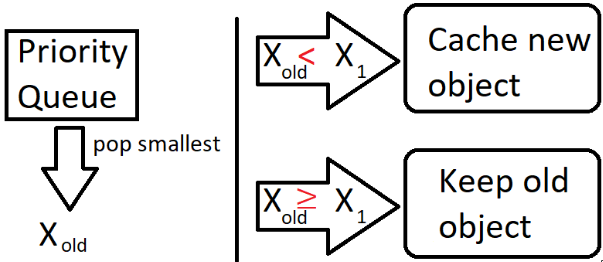
\includegraphics[width=0.75\linewidth]{pics/cache2.png}
	\caption{Usage of prediction by the policy.}
	\label{fig:cache2}
\end{figure}

After the prediction is made, the value $X_1$ is used to decide if the object should be put in the cache. The policy maintains a priority queue in which the key of each entry is the predicted popularity, and the values are IDs of the objects currently stored in the cache. When a new object is requested, and it has not been stored in the cache, the neural network predicts the popularity of the object in the future - $X_1$. Then, an object with the smallest predicted popularity is fetched from the priority queue, and its popularity is denoted as $X_{old}$. If the value $X_1$ is greater than $X_{old}$, then the old object is removed from the cache, and the new one is put in its place and into the priority queue. Otherwise, no change occurs. 

With this design, a problem may arise - if the prediction of popularity for some object has been calculated to be very high, it may never be removed from the cache since it will never be fetched for replacement. A solution to this problem is to update the priority for a few random objects stored in the cache with each cache hit.

\begin{figure}[t!]
	\centering
	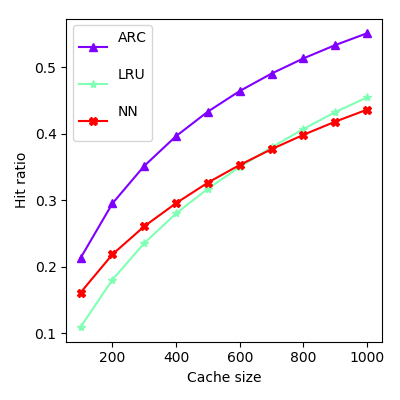
\includegraphics[width=0.5\linewidth]{pics/cache3.png}
	\caption{Poor performance of the first version.}
	\label{fig:cache3}
\end{figure}

Also, the value $X_1$ requires a better explanation. Trying to predict the popularity of the object in the next time frame, as in the previous offline case, did not show good performance when evaluating the hit rate, as seen on the Figure \ref{fig:cache3}. The identified problem was that the prediction was made too far in the future. The influence of the issue can be summarized in two cases:

\begin{enumerate}
	\item If the object is popular in the current time window but then gets unpopular in the next, it wouldn't be put into the cache, but since the current time window is not finished, and the object is still popular, a lot of cache misses will occur.
	\item The opposite problem - when the object is not popular but then gets popular. This object will take a place in the cache even though it is not popular yet.
\end{enumerate}

To resolve this issue, we changed the scope of the value $X_1$. The desirable performance has been achieved with when $X_1$ represents the popularity at the end of the current time frame and displayed on the Figure \ref{fig:cache4}. Probably it is still possible to improve the performance by fine tuning the parameters. 

\begin{figure}[h!]
	\centering
	\begin{subfigure}[b]{0.49\linewidth}
		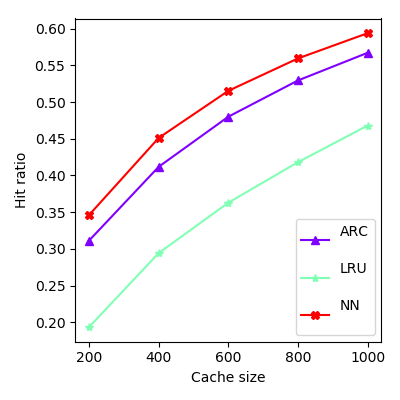
\includegraphics[width=\linewidth]{pics/cache4.png}
		\caption{5-day trace.}
	\end{subfigure}
	\begin{subfigure}[b]{0.49\linewidth}
		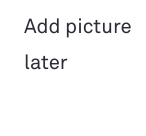
\includegraphics[width=\linewidth]{pics/todo.png}
		\caption{30-day trace.}
	\end{subfigure}
	\caption{Improved performance of the policy.}
	\label{fig:cache4}
\end{figure}

\subsection{Online learning}

One of the most important parts of a caching policy is to be able to perform well in different environments with different traffic patterns. That is why it is important to make the policy adaptable. In our case, such adaptability is provided by the ability of the neural network to continuously evolve by training on the newly arrived data. After the end of each time frame, it is possible to generate a new training dataset and use it to train the neural network, possibly asynchronously. But by training only on the latest data, we may encounter the problem of catastrophic forgetting\cite{16, 17}. In short, the issue is that by training only on the latest data the neural network will forget the information about the old underlying relations between input and output even though they still may be relevant for predictions. 

To overcome this issue, we incorporate a technique of keeping the training datasets of previous time frames and training the neural network also on them. But since they represent less relevant data, the error, which is backpropagated during the training of the neural network, is scaled down with a parameter $\alpha^M \text{, where } 0 < \alpha < 1 \text{ and } M$ - is the distance from current time frame to previous time frames. In this way, the error on the latest data will stay unchanged since the value of $M$ is $0$. Moving further in the past $\alpha^M \rightarrow 0$ and the influence of the old data is reduced. When $\alpha^M$ reaches some small value, the old training data becomes too irrelevant and can be removed from the memory. Using this approach with the value of $\alpha = 0.5$ and forget threshold of $0.001$ it is required to store training datasets generated only for $10$ latest time frames while keeping the predictions made by the neural network accurate and relevant.

\subsection{Parameter selection}

Having achieved good performance on the real 5-day trace and overperforming state of the art policy ARC on all cache sizes, as seen in the Figure \ref{fig:cache4}, even without giving much consideration to the parameters of the proposed policy, it is time to explore the optimal ways to select the parameters.

\begin{figure}[b!]
	\centering
	
	\begin{subfigure}[b]{0.49\linewidth}
		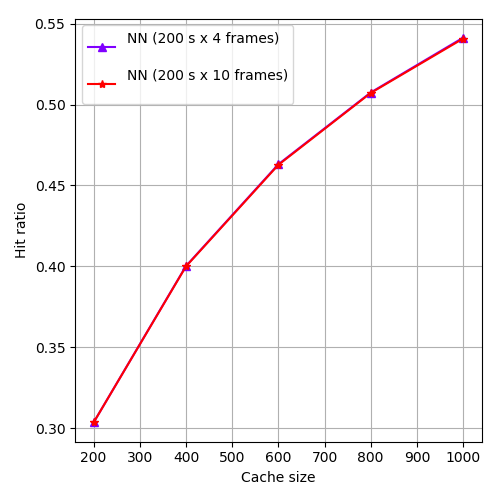
\includegraphics[width=\linewidth]{pics/cache5.png}
		\caption{5-day trace.}
	\end{subfigure}
	\begin{subfigure}[b]{0.49\linewidth}
		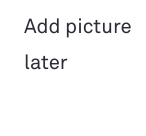
\includegraphics[width=\linewidth]{pics/todo.png}
		\caption{30-day trace.}
	\end{subfigure}
	\caption{Comparison of performance with larger number of time frames.}
	\label{fig:cache5}
\end{figure}

The first step we decided to check is the required number of time windows. To establish this experiment, we have fixed the length of the time frame at the values of 200 seconds and tested two configurations - 4 time frames (3 previous + current) and 10 time frames (9 previous + current). The results of the experiment can be seen in the Figure \ref{fig:cache5}. As seen in the figure, the cache hit ratio values coincide for each tested cache size. From this, we can conclude that it is enough to use 4 time frames for popularity predictions and there is no point in increasing this number.


Following this, we have to determine the optimal way to select the length of the time frame. We have established an experiment trying to evaluate this value. Parameters of the experiment:

\begin{itemize}
	\item Time frame sizes: 3 s, 10 s, 50 s, 200 s, 1000 s.
	\item Cache sizes: 200, 400, 600, 800, 1000.
	\item Trace length: first 50 000 000 requests from both of real traces.
\end{itemize}

\begin{figure}[t!]
	\centering
	
	\begin{subfigure}[b]{0.49\linewidth}
		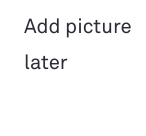
\includegraphics[width=\linewidth]{pics/todo.png}
		\caption{5-day trace.}
	\end{subfigure}
	\begin{subfigure}[b]{0.49\linewidth}
		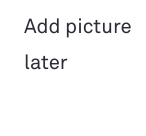
\includegraphics[width=\linewidth]{pics/todo.png}
		\caption{30-day trace.}
	\end{subfigure}
	\caption{Comparison of performance with different size of time frame.}
	\label{fig:cache6}
\end{figure}

The experiment showed that the size of the window influences more on the performance than the number of windows. For both traces, the size of 200 s showed the best performance for all cache sizes, as you can observe on the Figure \ref{fig:cache6}. From this, we can propose a rule of thumb for selecting the size of the time frame for the policy. It is reasonable to assume that the lower the request rate the higher the size of the time frame should be, since with fixed length of the time frame and decreasing request rate the accuracy of the estimation of the popularity of the objects also decreases. Both traces have approximately 900 requests/s request rate and show the best performance at the size of the window of 200 s. Thus, the rule of thumb is to select the size of the window such that the next equation holds true: $$ frame\_size * request\_rate \approx  180000 $$.